% !TeX encoding = UTF-8

%% ------------------------------------------------------------------------
%% Copyright (C) 2021 SJTUG
%% 
%% SJTUBeamer Example Document by SJTUG
%% 
%% SJTUBeamer Example Document is licensed under a
%% Creative Commons Attribution-NonCommercial-ShareAlike 4.0 International License.
%% 
%% You should have received a copy of the license along with this
%% work. If not, see <http://creativecommons.org/licenses/by-nc-sa/4.0/>.
%% -----------------------------------------------------------------------

\documentclass[xcolor=table,dvipsnames,svgnames,aspectratio=169]{ctexbeamer}
% 可以通过 fontset=macnew / fontset=ubuntu / fontset=windows 选项切换字体集

\usepackage{tikz}
\usepackage[normalem]{ulem}
\usetikzlibrary{arrows}
\usepackage{amsmath}
\usepackage{mflogo}
\usepackage{graphicx}
\usepackage{xspace}
\usepackage{amsmath}
\usepackage{unicode-math}
\usepackage{ccicons}
\usepackage{hologo}
\usepackage{colortbl}
\usepackage{shapepar}
\usepackage{hyperxmp}
\usepackage{booktabs}
\usepackage{qrcode}
\usepackage{listings}
\usepackage{tipa}
\usepackage{multicol}
\usepackage{datetime2}
\usepackage{fontawesome5}
\usepackage{hyperref}
\usepackage[backend=biber,style=gb7714-2015]{biblatex}

\addbibresource{thesis.bib}
\setbeamertemplate{bibliography item}[text]

\graphicspath{{figures/}}

\hypersetup{
  pdfsubject = {PhD-ResearchProposal},
  pdfauthor = {Pedro Hernández Rubio},
  pdfcopyright = {Licensed under CC-BY-SA 4.0. Some rights reserved.},
  pdflicenseurl = {http://creativecommons.org/licenses/by-sa/4.0/},
  unicode            = true,
  psdextra           = true,
  pdfdisplaydoctitle = true
}

\pdfstringdefDisableCommands{
  \let\\\relax
  \let\quad\relax
  \let\hspace\@gobble
}

\renewcommand{\TeX}{\hologo{TeX}}
\renewcommand{\LaTeX}{\hologo{LaTeX}}
\newcommand{\BibTeX}{\hologo{BibTeX}}
\newcommand{\XeTeX}{\hologo{XeTeX}}
\newcommand{\pdfTeX}{\hologo{pdfTeX}}
\newcommand{\LuaTeX}{\hologo{LuaTeX}}
\renewcommand{\CTeX}{C\TeX}
\newcommand{\MiKTeX}{\hologo{MiKTeX}}
\newcommand{\MacTeX}{Mac\hologo{TeX}}
\newcommand{\beamer}{\textsc{beamer}}
\newcommand{\XeLaTeX}{\hologo{Xe}\kern-.13em\LaTeX{}}
\newcommand{\pdfLaTeX}{pdf\LaTeX{}}
\newcommand{\LuaLaTeX}{Lua\LaTeX{}}

\def\TeXLive{\TeX{} Live\xspace}
\let\TL=\TeXLive
\newcommand{\SJTUThesis}{\textsc{SJTUThesis}\xspace}
\newcommand{\SJTUBeamer}{\textsc{SJTUBeamer}\xspace}
\newcommand{\SJTUThesisVersion}{1.0.0rc7}
\newcommand{\SJTUThesisDate}{2020/7/31}

\newcommand\link[1]{\href{#1}{\faLink}}
\newcommand\pkg[1]{\texttt{#1}}

\def\cmd#1{\texttt{\color{DarkBlue}\footnotesize $\backslash$#1}}
\def\env#1{\texttt{\color{DarkBlue}\footnotesize #1}}
\def\cmdxmp#1#2#3{\small{\texttt{\color{DarkBlue}$\backslash$#1}\{#2\}\hspace{1em}\\ $\Rightarrow$\hspace{1em} {#3}\par\vskip1em}}

\lstset{
  language=[LaTeX]TeX,
  basicstyle=\ttfamily\footnotesize,
  tabsize=2,
  keywordstyle=\bfseries\ttfamily\color{cprimary},
  commentstyle=\sl\ttfamily\color[RGB]{100,100,100},
  stringstyle=\ttfamily\color[RGB]{50,50,50},
  extendedchars=true,
  breaklines=true,
}

\lstdefinestyle{style@inline}{
  basicstyle   = \ttfamily,
  keepspaces   = true
}
\lstMakeShortInline[style=style@inline]|

\usetheme[max, red, light, infolines]{sjtubeamer}
% 使用 maxplus/max/min 切换标题页样式
% 使用 red/blue 切换主色调
% 使用 light/dark 切换亮/暗色模式
% 使用外样式关键词以获得不同的边栏样式
%   miniframes infolines  sidebar* 
%   default    smoothbars split	 
%   shadow     tree       smoothtree
% *siderbar 推荐与 max 一起使用。

% \tikzexternalize[prefix=cache/]
% 如果您需要缓存 tikz 图像,请取消注释上一行,并在编译选项中添加 -shell-escape。

\author{Hugo Vanhille, Pedro Hernández Rubio}
\institute[SEIEE]{Department of Automation}
\date{\the\year 年 \the\month 月}
\subject{ECE6903J - Distributed Machine Learning Systems}
\title{Blockchain-based Federated Learning: privacy and incentive}
\title[DMLS] % 页脚显示标题
{\textbf{Blockchain-based Federated Learning: privacy and incentive}} % 首页标题

\subtitle{ECE6903J - Distributed Machine Learning Systems (Research project)}
%\subtitle{Evaluation of blockchain technology in student mobility administration process}

\begin{document}

% 使用节目录
\AtBeginSection[]{
  \begin{frame}
    % \tableofcontents[currentsection]           % 传统节目录             
    \sectionpage                   % 节页
  \end{frame}
}

% 使用小节目录
\AtBeginSubsection[]{                  % 在每小节开始
  \begin{frame}
    % \tableofcontents[currentsection,currentsubsection]             % 传统小节目录             
    \subsectionpage                % 小节页
  \end{frame}
}

\maketitle

\begin{frame}{目录}
\begin{multicols}{2}
  \tableofcontents
  \end{multicols}
\end{frame}

% !TeX encoding = UTF-8
% !TeX root = ../main.tex

%% ------------------------------------------------------------------------
%% Copyright (C) 2021 SJTUG
%% 
%% SJTUBeamer Example Document by SJTUG
%% 
%% SJTUBeamer Example Document is licensed under a
%% Creative Commons Attribution-NonCommercial-ShareAlike 4.0 International License.
%% 
%% You should have received a copy of the license along with this
%% work. If not, see <http://creativecommons.org/licenses/by-nc-sa/4.0/>.
%% -----------------------------------------------------------------------

\section{Background}

\subsection{Motivation}

\begin{frame}{Motivation}
	\begin{block}{Goal}
        Applying ML to systems (blockchain-based models)
      \end{block}
  \begin{itemize}
    \item Research line mainly targeted to \alert{blockchain technology} (its application to systems)
    \item Research group in Department of Automation (PhD supervisors) has been recently working in blockchain-based models applied to \alert{trust management systems}
	\item Specifically, applied to data-aggregation systems in the Internet of Things (IoT) field \alert{crowdsensing}
	\item Could similar approach be applied for \alert{Federated Learning}?
%    \item My PhD thesis could use some of the model simulation techniques (stochastic processes) used in this research paper experimentation
%    \item And of course, it is related to a emerging subfield that could greatly contribute to the development of the Internet of Things (IoT)
  \end{itemize}
\end{frame}

\subsection{Crowdsensing}

\begin{frame}{Crowdsensing: definition}
  \begin{itemize}
  \item \textbf{Crowdsensing:} emerging paradigm of data aggregation\cite{paper1}, having a key role in data-driven applications. Specially used for getting large ammounts of IoT sensing data, by using the individual intelligent sensing devices.
  \item \textbf{Benefit:} improved data collection efficiency and reduced costs effectively\cite{paper2}
  \end{itemize}
  \begin{figure}[h]
        \centering
        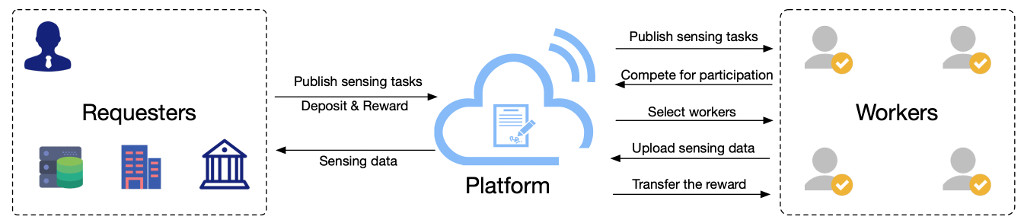
\includegraphics[width=.8\textwidth]{201909-wei-figure1.jpg}
      \end{figure}
\end{frame}

\begin{frame}{Crowdsensing: issues}
  		\begin{enumerate}
   			\item Managed and maintained \alert{centralized platforms} suffer from the single point of failure
   				\begin{itemize}
   					\item \textbf{Proposal: } decentralized architecture (blockchain technology) that lacks a single point of failure, and enhances privacy with asymmetric encryption and digital signature technology
   				\end{itemize}
    		\item Encouraging workers by offering appropiate \alert{incentive mechanisms} (monetary usually) \rightarrow  \underline{auction theory} guarantees benefits for both requesters and workers\cite{paper15} but only provide short-term incentives
    			\begin{itemize}
   					\item \textbf{Proposal:} hybrid incentive mechanism, adopting \underline{mechanism design theory}, considering three factors:
   					\begin{itemize}
   					\item Monetary reward
   					\item Reputation evaluation
   					\item Data quality
   					\end{itemize}
   				\end{itemize}
  		\end{enumerate}
\end{frame}

%% !TeX encoding = UTF-8
% !TeX root = ../main.tex

%% ------------------------------------------------------------------------
%% Copyright (C) 2021 SJTUG
%% 
%% SJTUBeamer Example Document by SJTUG
%% 
%% SJTUBeamer Example Document is licensed under a
%% Creative Commons Attribution-NonCommercial-ShareAlike 4.0 International License.
%% 
%% You should have received a copy of the license along with this
%% work. If not, see <http://creativecommons.org/licenses/by-nc-sa/4.0/>.
%% -----------------------------------------------------------------------

\section{Introduction}

\subsection{Background}

%\begin{frame}{Motivation}
%  Reasons behind my research paper choice:
%  \begin{itemize}
%    \item My research line is mainly targeted to blockchain technology
%    \item This specific research paper has been developed by my PhD co-supervisors (good chance to learn about their researching style)
%    \item My PhD thesis could use some of the model simulation techniques (stochastic processes) used in this research paper experimentation
%    \item And of course, it is related to a emerging subfield that could greatly contribute to the development of the Internet of Things (IoT)
%  \end{itemize}
%\end{frame}

\begin{frame}[fragile]{Background}

  Blockchain technology $\rightarrow$ theoretical potential:
  \begin{itemize}
		\item Data integrity
		\item Decentralizing trust
		\item Reducing costs
  \end{itemize}
	
  Useful practical application? $\rightarrow$ \alert{e-government} (software administration processes)
    
   \begin{exampleblock}{From generic case to more specific}
    	\textbf{studenty mobility management} $\subset$ supply chain management
  \end{exampleblock}

\end{frame}

%\subsection{Crowdsensing}
%
%\begin{frame}{Crowdsensing: definition}
%  \begin{itemize}
%  \item \textbf{Crowdsensing:} emerging paradigm of data aggregation\cite{paper1}, having a key role in data-driven applications. Specially used for getting large ammounts of IoT sensing data, by using the individual intelligent sensing devices.
%  \item \textbf{Benefit:} improved data collection efficiency and reduced costs effectively\cite{paper2}
%  \end{itemize}
%  \begin{figure}[h]
%        \centering
%        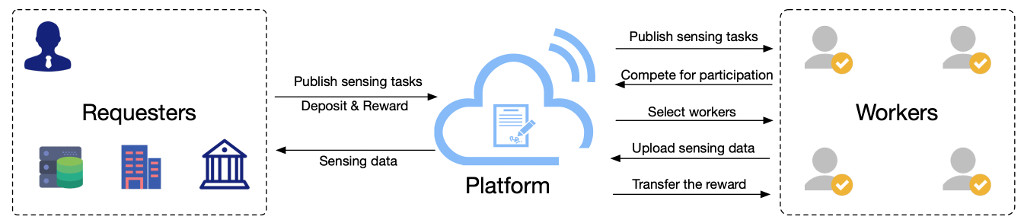
\includegraphics[width=.8\textwidth]{201909-wei-figure1.jpg}
%      \end{figure}
%\end{frame}
%
%\begin{frame}{Crowdsensing: issues}
%  		\begin{enumerate}
%   			\item Managed and maintained \alert{centralized platforms} suffer from the single point of failure
%   				\begin{itemize}
%   					\item \textbf{Proposal: } decentralized architecture (blockchain technology) that lacks a single point of failure, and enhances privacy with asymmetric encryption and digital signature technology
%   				\end{itemize}
%    		\item Encouraging workers by offering appropiate \alert{incentive mechanisms} (monetary usually) \rightarrow  \underline{auction theory} guarantees benefits for both requesters and workers\cite{paper15} but only provide short-term incentives
%    			\begin{itemize}
%   					\item \textbf{Proposal:} hybrid incentive mechanism, adopting \underline{mechanism design theory}, considering three factors:
%   					\begin{itemize}
%   					\item Monetary reward
%   					\item Reputation evaluation
%   					\item Data quality
%   					\end{itemize}
%   				\end{itemize}
%  		\end{enumerate}
%\end{frame}

% !TeX encoding = UTF-8
% !TeX root = ../main.tex

%% ------------------------------------------------------------------------
%% Copyright (C) 2021 SJTUG
%% 
%% SJTUBeamer Example Document by SJTUG
%% 
%% SJTUBeamer Example Document is licensed under a
%% Creative Commons Attribution-NonCommercial-ShareAlike 4.0 International License.
%% 
%% You should have received a copy of the license along with this
%% work. If not, see <http://creativecommons.org/licenses/by-nc-sa/4.0/>.
%% -----------------------------------------------------------------------

\section{Research}

\subsection{Problems}

%\begin{frame}{Research problems}
%\begin{enumerate}
%\item Organizational \textbf{P2P networks} (universities message system): \alert{efficiency?} (messaging time spent and memory space used) $\rightarrow$ \textbf{energy sustainability?}
%\item University network connections (graph theory): \textbf{predicting and recommending partners}: trust? $\rightarrow$ \textbf{links reliability?} \alert{(Machine Learning techniques)}
%\item \textbf{Competitive application calls}: \alert{auction theory (mechanism design)} auditability? $\rightarrow$ \textbf{meritocracy?}
%\end{enumerate}
%\begin{alertblock}{Research studies on practical applications?}
%So far, plenty of theoretical research on blockchain technologies but lack of empirical evidence on real-world practical applications (non-mature and complex technology)
%\end{alertblock}
%\end{frame}

\subsection{The privacy-preserving of Federated Learning}
\begin{frame}{The privacy-preserving of Federated Learning}
    \begin{itemize}
        \item FL provides an attractive structure for decomposing the overall machine learning workflow into the approachable modular units we desire.%(presented in (Kairouz et al.))
        \item FL provides a level of privacy to participating users through data minimization.
    \end{itemize}
    \begin{figure}[h]
        \centering
        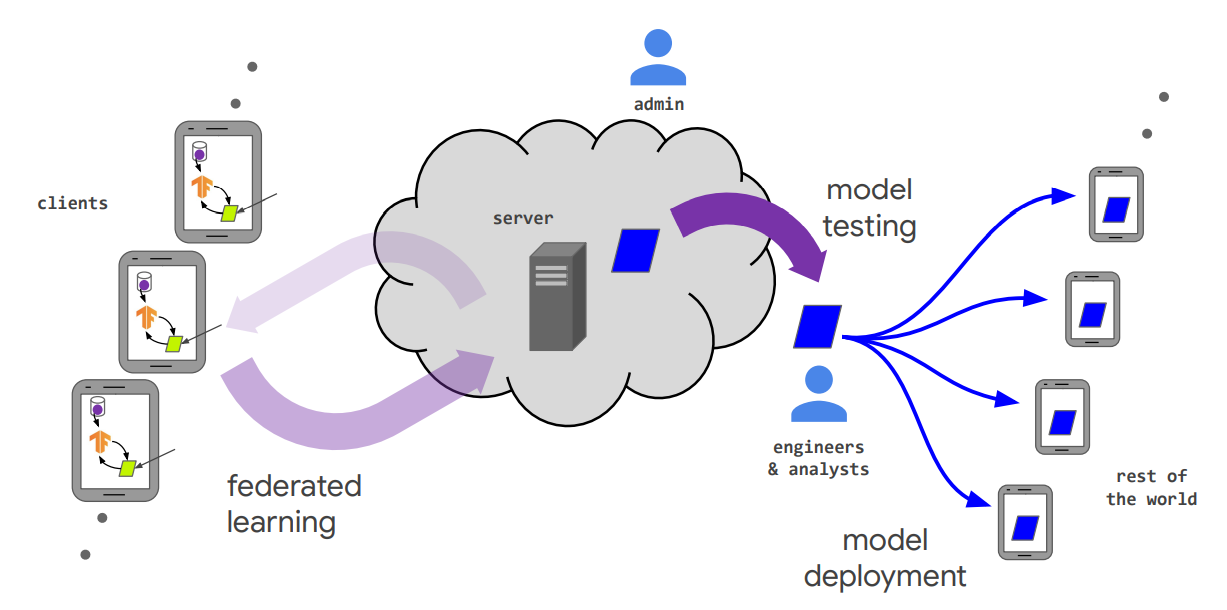
\includegraphics[width=8cm]{structureFL.PNG}
    \end{figure}
\end{frame}

\subsection{The incentive mechanism of Federated Learning}
\begin{frame}{The incentive mechanism of Federated Learning}
  \begin{itemize}
    \item Main types of incentive mechanisms:
          \begin{enumerate}
            \item \alert{Monetary-based}: distributing rewards. %And two subtypes can be considered\cite{paper16}:
            	% \begin{itemize}
            	% \item \alert{price-decision-first} (auction theory) design optimal mechanism benefiting both requesters adn workers
            	% \item \alert{upload-decision-first}: distributing rewards base on the uploaded data (quality)
          		% \end{itemize}
            \item \alert{Reputation-based}: reputation framework for worker selection (algorithms)
          \end{enumerate}
    \item \textbf{Limitations}
    	\begin{enumerate}
            \item Relies on a central platform, vulnerable to target attacks
            \item Single-attribute incentive mechanisms (multifactor incentive needed)
          \end{enumerate}
     %Some previous hybrid incentive mechanisms\cite{paper52} suffer of usability problems because the difficulty of hybrid data management
  \end{itemize}
\end{frame}

%\section{Research}
%
%\subsection{Problems}
%
%\begin{frame}{Blockchain background}
%  \alert{Distributed ledger containing a time-stamped series of immutable blockchains, trustless, decentralized, proof-tampering and full traceability}
%%   \begin{itemize}
%%     \item Research approaches on blockchain-based crowdsensing:
%%           \begin{itemize}
%%             \item Evaluating time consumption and task cost of applying a blockchain-based system\cite{paper33}
%%             \item Blockchain-based crowdsensing quality control model\cite{paper34}
%%             \item Considering privacy issues\cite{paper35}
%%             \item Handling location privacy protection\cite{paper37} (confusion mechanism)
%%           \end{itemize}
%%   \end{itemize}
%    \begin{figure}[h]
%        \centering
%        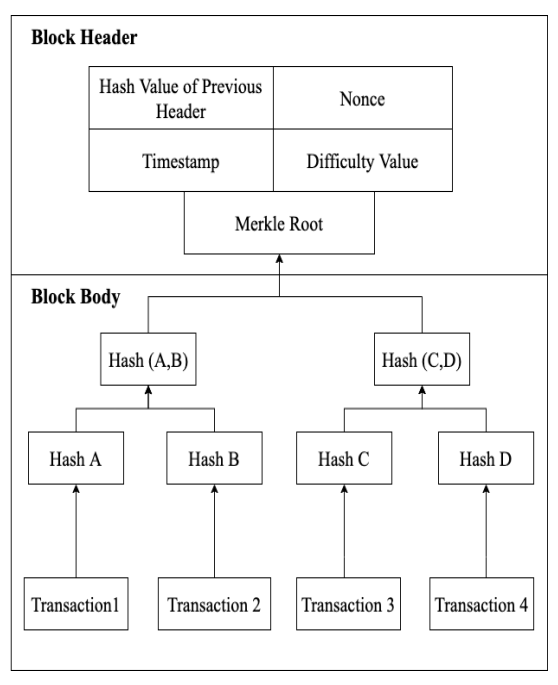
\includegraphics[width=8cm]{topologyBC.PNG}
%    \end{figure}
%\end{frame}
%
%%\begin{frame}{Research problems}
%%\begin{enumerate}
%%\item Organizational \textbf{P2P networks} (universities message system): \alert{efficiency?} (messaging time spent and memory space used) $\rightarrow$ \textbf{energy sustainability?}
%%\item University network connections (graph theory): \textbf{predicting and recommending partners}: trust? $\rightarrow$ \textbf{links reliability?} \alert{(Machine Learning techniques)}
%%\item \textbf{Competitive application calls}: \alert{auction theory (mechanism design)} auditability? $\rightarrow$ \textbf{meritocracy?}
%%\end{enumerate}
%%\begin{alertblock}{Research studies on practical applications?}
%%So far, plenty of theoretical research on blockchain technologies but lack of empirical evidence on real-world practical applications (non-mature and complex technology)
%%\end{alertblock}
%%\end{frame}
%
%\subsection{The privacy-preserving of crowdsensing}
%\begin{frame}{The privacy-preserving of crowdsensing}
%    \begin{itemize}
%        \item FL provides an attractive structure (presented in (Kairouz et al.)) for decomposing the overall machine learning workflow into the approachable modular units we desire.
%        \item FL provides a level of privacy to participating users through data minimization.
%    \end{itemize}
%    \begin{figure}[h]
%        \centering
%        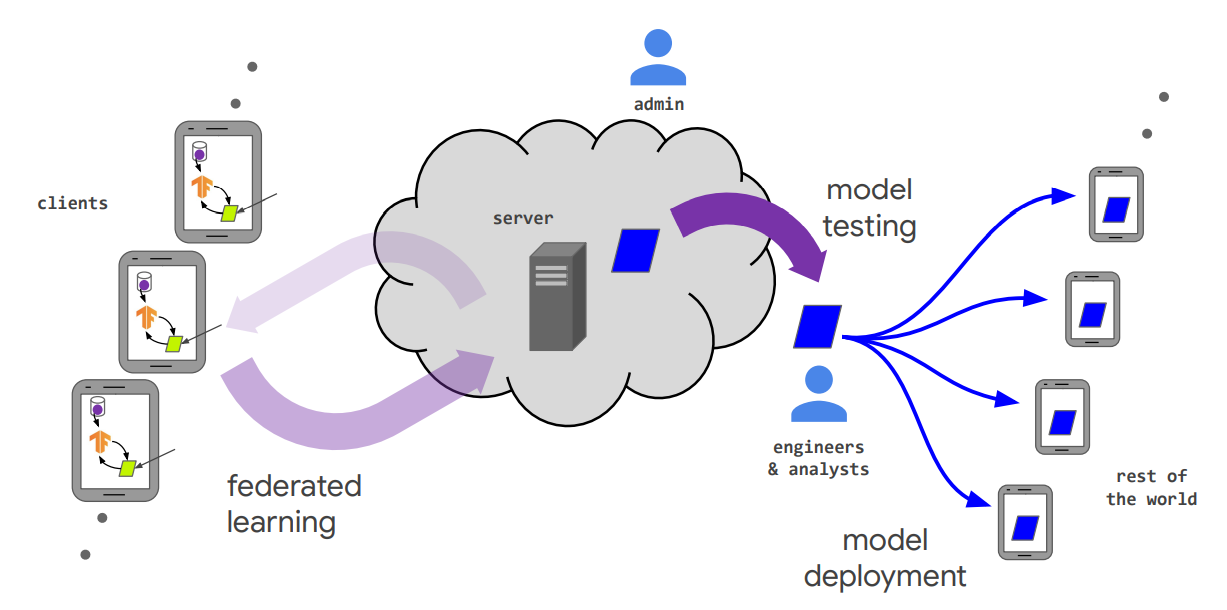
\includegraphics[width=8cm]{structureFL.PNG}
%    \end{figure}
%\end{frame}
%
%\subsection{The incentive mechanism of crowdsensing}
%\begin{frame}{The incentive mechanism of crowdsensing}
%  \begin{itemize}
%    \item Main types of incentive mechanisms:
%          \begin{enumerate}
%            \item \alert{Monetary-based}: distributing rewards. %And two subtypes can be considered\cite{paper16}:
%            	% \begin{itemize}
%            	% \item \alert{price-decision-first} (auction theory) design optimal mechanism benefiting both requesters adn workers
%            	% \item \alert{upload-decision-first}: distributing rewards base on the uploaded data (quality)
%          		% \end{itemize}
%            \item \alert{Reputation-based}: reputation framework for worker selection (algorithms)
%          \end{enumerate}
%    \item \textbf{Limitations}
%    	\begin{enumerate}
%            \item Relies on a central platform, vulnerable to target attacks
%            \item Single-attribute incentive mechanisms (multifactor incentive needed)
%          \end{enumerate}
%     %Some previous hybrid incentive mechanisms\cite{paper52} suffer of usability problems because the difficulty of hybrid data management
%  \end{itemize}
%\end{frame}
%
%%\section{Research}
%%
%%\subsection{Problems}
%%
%%\begin{frame}{Blockchain background}
%%  \alert{Distributed ledger containing a time-stamped series of immutable blockchains, trustless, decentralized, proof-tampering and full traceability}
%%  \begin{itemize}
%%    \item Research approaches on blockchain-based crowdsensing:
%%          \begin{itemize}
%%            \item Evaluating time consumption and task cost of applying a blockchain-based system\cite{paper33}
%%            \item Blockchain-based crowdsensing quality control model\cite{paper34}
%%            \item Considering privacy issues\cite{paper35}
%%            \item Handling location privacy protection\cite{paper37} (confusion mechanism)
%%          \end{itemize}
%%  \end{itemize}
%%\end{frame}
%%
%%%\begin{frame}{Research problems}
%%%\begin{enumerate}
%%%\item Organizational \textbf{P2P networks} (universities message system): \alert{efficiency?} (messaging time spent and memory space used) $\rightarrow$ \textbf{energy sustainability?}
%%%\item University network connections (graph theory): \textbf{predicting and recommending partners}: trust? $\rightarrow$ \textbf{links reliability?} \alert{(Machine Learning techniques)}
%%%\item \textbf{Competitive application calls}: \alert{auction theory (mechanism design)} auditability? $\rightarrow$ \textbf{meritocracy?}
%%%\end{enumerate}
%%%\begin{alertblock}{Research studies on practical applications?}
%%%So far, plenty of theoretical research on blockchain technologies but lack of empirical evidence on real-world practical applications (non-mature and complex technology)
%%%\end{alertblock}
%%%\end{frame}
%%
%%\subsection{The privacy-preserving of crowdsensing}
%%
%%\subsection{The incentive mechanism of crowdsensing}
%%
%%\begin{frame}{The incentive mechanism of crowdsensing}
%%  \begin{itemize}
%%    \item Main types of incentive mechanisms:
%%          \begin{enumerate}
%%            \item \alert{Monetary-based}: distributing rewards. And two subtypes can be considered\cite{paper16}:
%%            	\begin{itemize}
%%            	\item \alert{price-decision-first} (auction theory) design optimal mechanism benefiting both requesters adn workers
%%            	\item \alert{upload-decision-first}: distributing rewards base on the uploaded data (quality)e
%%          		\end{itemize}
%%            \item \alert{Reputation-based}: reputation framework for worker selection (algorithms)
%%          \end{enumerate}
%%    \item \textbf{Limitations}
%%    	\begin{enumerate}
%%            \item Relies on a central platform, vulnerable to target attacks
%%            \item Single-attribute incentive mechanisms (multifactor incentive needed)
%%          \end{enumerate}
%%     Some previous hybrid incentive mechanisms\cite{paper52} suffer of usability problems because the difficulty of hybrid data management
%%  \end{itemize}
%%\end{frame} %related
% !TeX encoding = UTF-8
% !TeX root = ../main.tex

%% ------------------------------------------------------------------------
%% Copyright (C) 2021 SJTUG
%% 
%% SJTUBeamer Example Document by SJTUG
%% 
%% SJTUBeamer Example Document is licensed under a
%% Creative Commons Attribution-NonCommercial-ShareAlike 4.0 International License.
%% 
%% You should have received a copy of the license along with this
%% work. If not, see <http://creativecommons.org/licenses/by-nc-sa/4.0/>.
%% -----------------------------------------------------------------------

\section{System architecture}

\subsection{Software application}

\begin{frame}{System architecture}
	\begin{figure}[h]
        \centering
        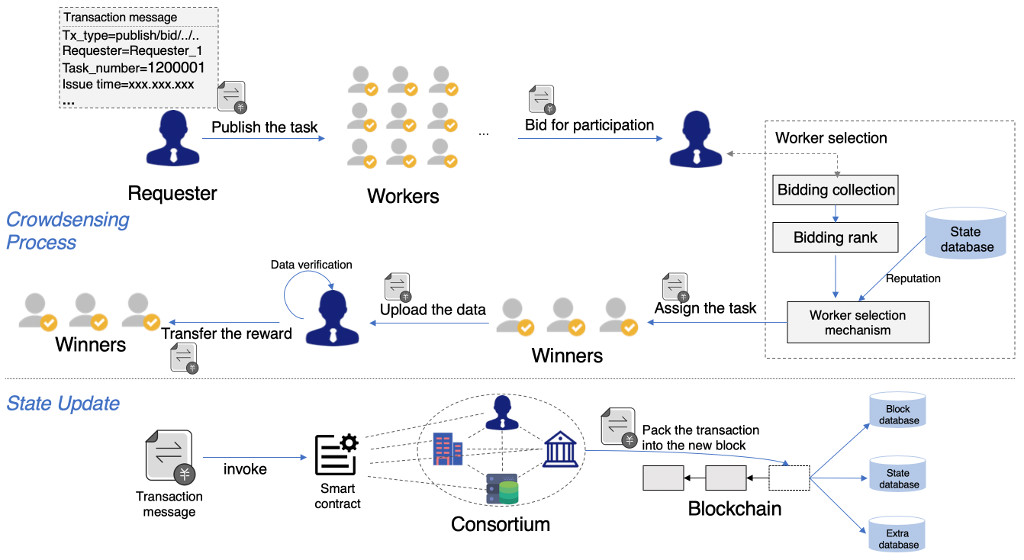
\includegraphics[width=.7\textwidth]{201909-wei-figure2.jpg}
      \end{figure}
\end{frame}

%\begin{frame}{Blockchain application}
%\begin{columns}[T,onlytextwidth]
%    \column{0.7\textwidth}
%	\begin{center}
%		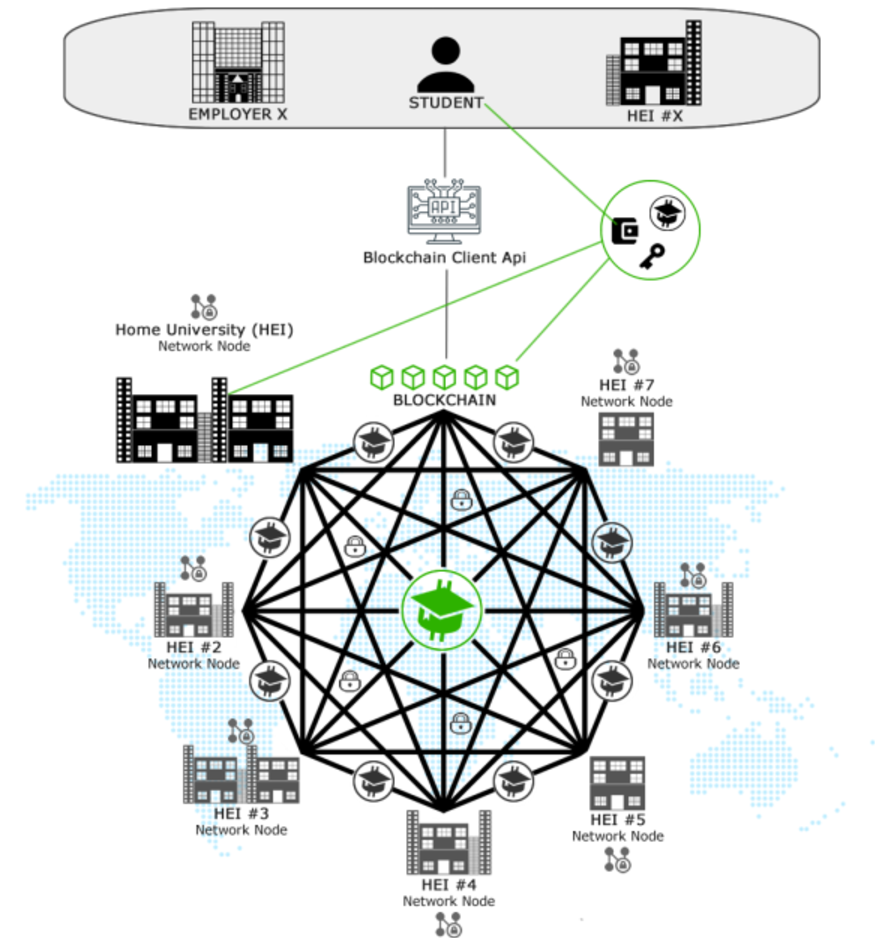
\includegraphics[height=.8\textheight]{eductx.pdf}\hfill
%	\end{center}
%	\column{0.3\textwidth}
%%	\metroset{block=fill}
%      \begin{exampleblock}{Platform}
%        Ethereum
%      \end{exampleblock}
%      \begin{exampleblock}{NF tokens}
%        University credits
%      \end{exampleblock}
%      \begin{exampleblock}{Consensus}
%        Proof-of-stake
%      \end{exampleblock}
%      \begin{exampleblock}{Scope}
%        Public
%      \end{exampleblock}
%      \begin{exampleblock}{Licence}
%        Open source
%      \end{exampleblock}
%\end{columns}
%\end{frame}

%\begin{frame}{Blockchain application}
%  \begin{columns}[c]
%    \begin{column}{.45\textwidth}
%      \begin{itemize}
%        \item Platform
%              \begin{itemize}
%                \item Ethereum
%                \item Hyperledger
%              \end{itemize}
%        \item NF tokens: exchange students
%        \item Consensus: proof-of-stake
%        \item Scope: public
%		\item License: open source
%      \end{itemize}
%    \end{column}
%    \begin{column}{.45\textwidth}
%      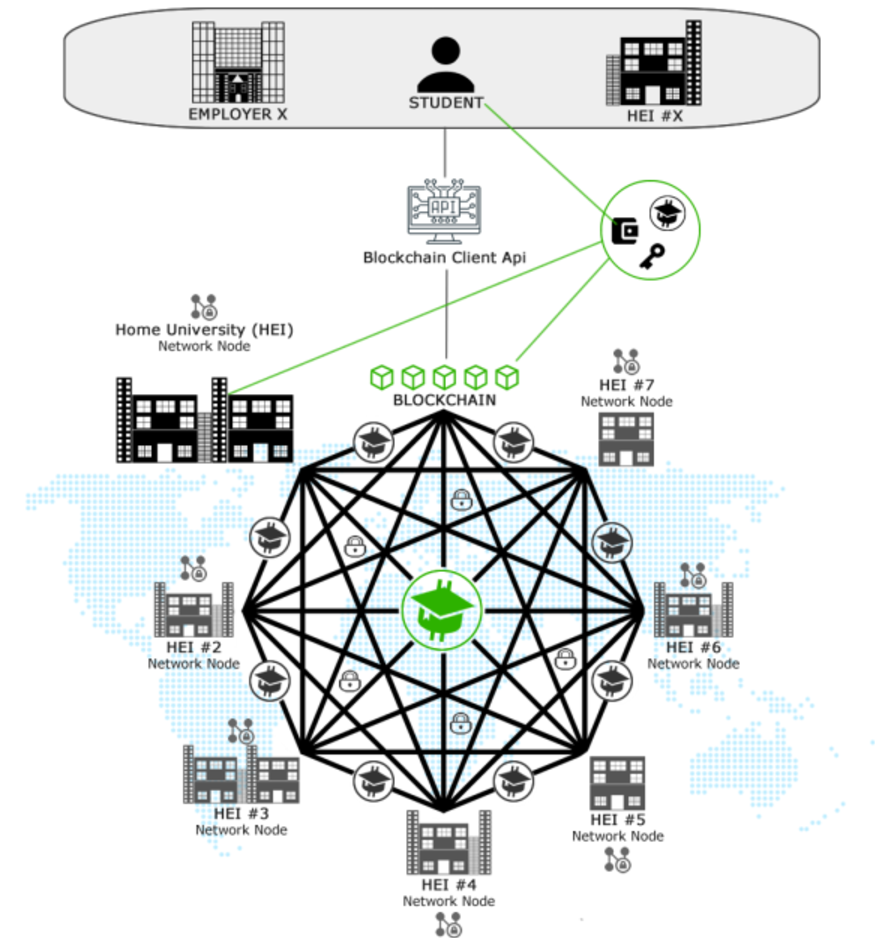
\includegraphics[width=\textwidth]{eductx.pdf}
%    \end{column}
%  \end{columns}
%\end{frame}

\begin{frame}{System flow}
  \begin{itemize}
    \item \textbf{System initialization}: configuration and identity authentication mechanisms
    \item \textbf{Task process}: Specific steps of crowdsensing
          \begin{itemize}
            \item Step 1: \alert{Task publishing} (invoking the smart contract to update the task state)
            \item Step 2: \alert{Worker selection} (workers submit the bidding price and workers select appropiate workers)
            \item Step 3: \alert{Data uploading} (selected workers perform the task and upload data)
            \item Step 4: \alert{Reward assignment and data evaluation} (requester distribute rewards and evaluate data quality)
          \end{itemize}
     \item \textbf{System synchronization}: state update about tasks and workers (validating transactions into new blocks)
  \end{itemize}
\end{frame}

% !TeX encoding = UTF-8
% !TeX root = ../main.tex

%% ------------------------------------------------------------------------
%% Copyright (C) 2021 SJTUG
%% 
%% SJTUBeamer Example Document by SJTUG
%% 
%% SJTUBeamer Example Document is licensed under a
%% Creative Commons Attribution-NonCommercial-ShareAlike 4.0 International License.
%% 
%% You should have received a copy of the license along with this
%% work. If not, see <http://creativecommons.org/licenses/by-nc-sa/4.0/>.
%% -----------------------------------------------------------------------

\section{Security issues: privacy}

\subsection{Provenance of data}

\begin{frame}{Provenance of data}
  \begin{exampleblock}{Model updates}
  A blockchain-based privacy-preserving federated learning framework leverages the immutability and decentralized trust properties of blockchain to provide the \alert{provenance of model updates} \textbf{(smart contracts)}
%  \item \textbf{Benefit:} improved data collection efficiency and reduced costs effectively
  \end{exampleblock}
  \begin{figure}[h]
        \centering
        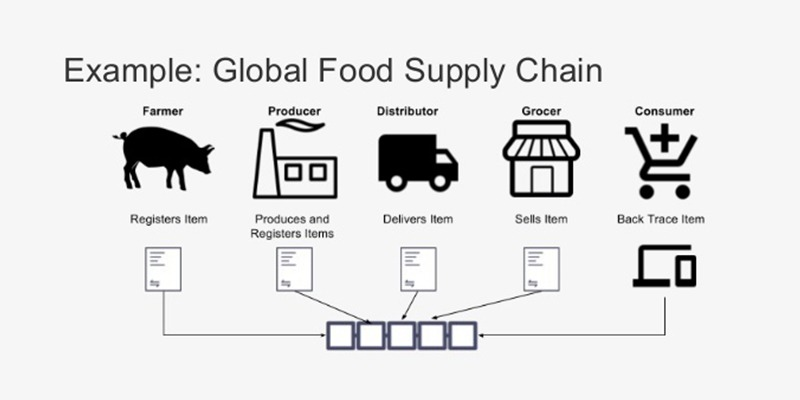
\includegraphics[width=.7\textwidth]{blockchain-in-supply-chain-industry-6.jpg}
      \end{figure}
\end{frame}

\subsection{Data privacy}

\begin{frame}{Data privacy}
\textbf{Improving data privacy in FL scenario:} 
\begin{itemize}
  		\item \alert{Storing evidence:} by using hashing and fingerprint mechanisms, references can be stored proving both local data and models are correct
  		\item \alert{Limiting access:} by making the ledger network only accessible via private network of participants
  		\item \alert{Zero Knowledge Proofs:} advanced (and computationally expensive) cryptographical techniques for granular information disclosure (both for mutual verification and partial data disclosure) 
\end{itemize}
\end{frame}

\section{Quality management: incentive}

\subsection{Incentive mechanism}

\begin{frame}{Incentive mechanism}
  \begin{exampleblock}{Federated Learning scenario}
 An effective incentive mechanism \alert{combining reputation with contract theory} motivates high-reputation mobile devices with high-quality data to participate in model learning
%  \item \textbf{Benefit:} improved data collection efficiency and reduced costs effectively
  \end{exampleblock}
  \begin{figure}[h]
        \centering
        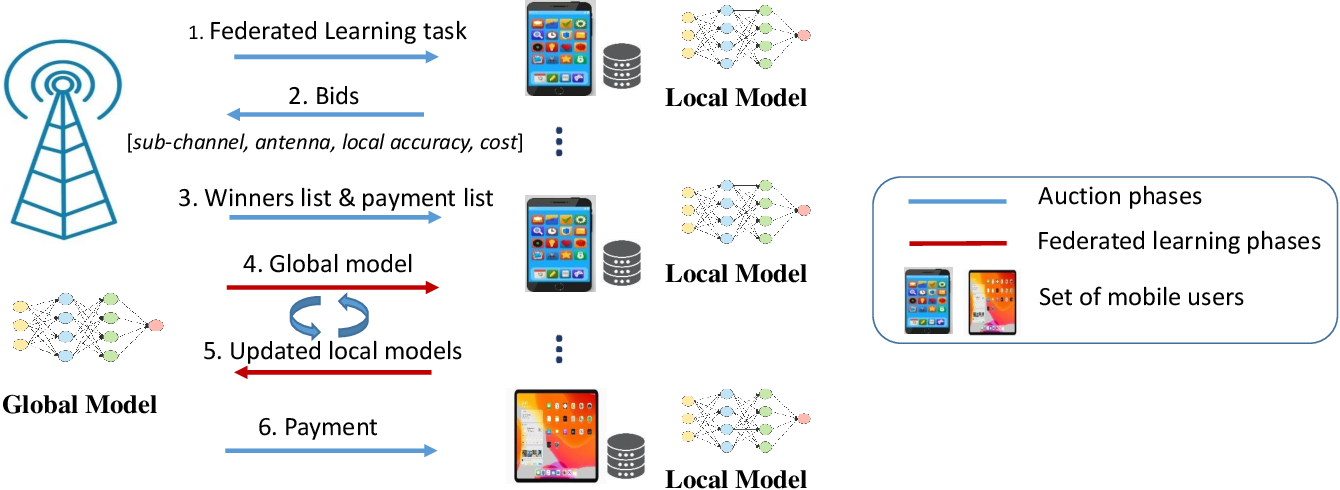
\includegraphics[width=.7\textwidth]{incentive-FL.png}
      \end{figure}
\end{frame}

%\subsection{1st research question}
%
%\begin{frame}{1st research question}
%	\begin{itemize}[<+- | alert@+>]
%		\item What are the differences between the use of standard networks and the use of
%blockchain networks in student mobility management in relation to the
%administration process efficiency?
%%		\metroset{block=fill}
%
%      \begin{block}{Goal}
%        Study the effects of blockchain technology in the field of student mobility
%management
%      \end{block}
%
%      \begin{block}{Methodology}
%        \emph{Quantitative:} Users activity logging (with and without blockchain)
%      \end{block}
%
%      \begin{block}{Analysis}
%        Social Network Analysis \& Web usage mining (logging)
%      \end{block}
%	\end{itemize}
%\end{frame}
%
%\subsection{2nd research question}
%
%\begin{frame}{2nd research question}
%	\begin{itemize}[<+- | alert@+>]
%		\item Following your paper on incentive model for crowdsensing\cite{electronics9020215}, I would like to explore how to use \alert{auction theory} and \alert{mechanism design theory} in a blockchain system, in order to identify an efficient model to assign exchange students to host universities (substituting classical competitive calls and applications).
%%		\metroset{block=fill}
%
%      \begin{block}{Goal}
%        Analyse the impact in student mobility competitive
%calls and applicants management
%      \end{block}
%
%      \begin{block}{Methodology}
%        \emph{Quantitative:} Several model simulations
%      \end{block}
%
%      \begin{block}{Analysis}
%        Effectiveness? Measure performance of several models
%      \end{block}
%	\end{itemize}
%\end{frame}
%
%\subsection{3rd research question}
%
%\begin{frame}{3rd research question}
%	\begin{itemize}[<+- | alert@+>]
%		\item Inter-universities agreements for student mobilites can be seen as a supply chain network: exchange students as assets. How to use \alert{machine learning} and \alert{predictive analytics} model, in a blockchain system, for better associations? Conflicts (geopolitical, pandemias, transport) alter mobilities feasibility. Effective planning?
%%		\metroset{block=fill}
%
%      \begin{block}{Goal}
%        Build a predictive model for optimal student mobility agreements
%      \end{block}
%
%      \begin{block}{Methodology}
%        \emph{Quantitative:} ratio of accomplished and failed mobilities
%      \end{block}
%
%      \begin{block}{Analysis}
%        Effectiveness? Measure performance of model in several scenarios
%      \end{block}
%	\end{itemize}
%\end{frame}

\subsection{Mechanism design: multifactor}

\begin{frame}{Mechanism design: multifactor}
  \begin{itemize}
    \item Based on three parameters:
          \begin{enumerate}
            \item \alert{Workers' bidding}
            \item \alert{Reputation}
            \item \alert{Recent data quality estimation}
          \end{enumerate}
    \item Analytic Hierarchy Process (AHP) framework \rightarrow (top-down)
    	\begin{enumerate}
            \item \alert{Objective level}: winning workers
            \item \alert{Criteria level}: parameters criteria
            \item \alert{Alternative level}: workers available
          \end{enumerate}
    \end{itemize}
    \begin{exampleblock}{Multifactor worker evaluation approach}
    	\begin{equation*}
      	\theta_{i}=\omega_{1} B_{i}+\omega_{2} R_{i}+\omega_{3} Q_{i} \quad\quad \text { where } \omega_{i} \geq 0 \text { and } \sum_{\omega_{i}=1}^{3} \omega_{i}=1	
    	\end{equation*}
  \end{exampleblock}
\end{frame}

\subsection{Mechanism design: issues}

\begin{frame}{Mechanism design: issues}
  		\begin{enumerate}
   			\item \textbf{How to select appropriate workers?}
   				\begin{itemize}
   					\item \textbf{Proposal: } decentralized architecture (blockchain technology) that lacks a single point of failure, and enhances privacy with asymmetric encryption and digital signature technology
   				\end{itemize}
    		\item \textbf{How to distribute the rewards to the workers?}
  		\end{enumerate}
  		With the help of \alert{mechanism design theory} two important properties for the incentive mechanism are guaranteed:
  		\begin{itemize}
   					\item \textbf{Incentive quality (IC):} the truthful submission of training cost is the worker's optimal bidding strategy
   					\item \textbf{Individual rationality (IR):} the reward must compensate for the worker's cost (non-negative)
   		\end{itemize}
\end{frame}
 %incentive
%% !TeX encoding = UTF-8
% !TeX root = ../main.tex

%% ------------------------------------------------------------------------
%% Copyright (C) 2021 SJTUG
%% 
%% SJTUBeamer Example Document by SJTUG
%% 
%% SJTUBeamer Example Document is licensed under a
%% Creative Commons Attribution-NonCommercial-ShareAlike 4.0 International License.
%% 
%% You should have received a copy of the license along with this
%% work. If not, see <http://creativecommons.org/licenses/by-nc-sa/4.0/>.
%% -----------------------------------------------------------------------

\section{Fieldwork} %Simulation and results

\subsection{Model simulation}

\begin{frame}{Model simulation}
	In order to validate the effectiveness of the proposed models, a number of experiments are executed to measure their performance:
  \begin{itemize}
	\item \alert{Internal Chinese student mobility program?} (students moving
to another chinese university during one academic year)
    \item Digital marketing: attract Chinese universities in order to
participante in experiments
    \item Involving \textbf{IROs} (International Relations Offices) officers and
IT staff into the use of experimental software applications →
acceptability issue?
	\item But quite hard to arrange! Better using some \alert{model simulation} techniques (stochastical
processes)

  \end{itemize}
\end{frame}
 %simulations
% !TeX encoding = UTF-8
% !TeX root = ../main.tex

%% ------------------------------------------------------------------------
%% Copyright (C) 2021 SJTUG
%% 
%% SJTUBeamer Example Document by SJTUG
%% 
%% SJTUBeamer Example Document is licensed under a
%% Creative Commons Attribution-NonCommercial-ShareAlike 4.0 International License.
%% 
%% You should have received a copy of the license along with this
%% work. If not, see <http://creativecommons.org/licenses/by-nc-sa/4.0/>.
%% -----------------------------------------------------------------------

\section{Conclusions}

\subsection{Application}

\begin{frame}{Results}
	A consortium blockchain-based incentive model for crowdsensing system is
proposed
  \begin{itemize}
  \item \textbf{Benefits of consortium blockchain technology:} 
  	\begin{itemize}
  		\item resistant to the single point of failure (system security)
  		\item cooperative management (by requesters) reduces cost and enhances the flexibility of the system (selection criteria)
  	\end{itemize}
  \item \textbf{Benefits of hybrid incentive mechanism:}
  	\begin{itemize}
  		\item encourages workers to contribute valuable data (and penalizes malicious ones)
  		\item ensures favorables short-term and long-term incentives for workers
  	\end{itemize}
  \end{itemize}
\end{frame}


\subsection{Limitations}

\begin{frame}{Limitations}
	Further research:
  \begin{enumerate}
  \item Dynamic situation where evaluations attributes are changing
  \item Optimization of consensus protocol (better performance)
  \item Further protection of worker privacy
  \end{enumerate}
  \begin{block}{Possible solutions}
  Application of ML techniques to blockchain-based system
  \end{block}
\end{frame}

\subsection{Further research}
%% !TeX encoding = UTF-8
% !TeX root = ../main.tex

%% ------------------------------------------------------------------------
%% Copyright (C) 2021 SJTUG
%% 
%% SJTUBeamer Example Document by SJTUG
%% 
%% SJTUBeamer Example Document is licensed under a
%% Creative Commons Attribution-NonCommercial-ShareAlike 4.0 International License.
%% 
%% You should have received a copy of the license along with this
%% work. If not, see <http://creativecommons.org/licenses/by-nc-sa/4.0/>.
%% -----------------------------------------------------------------------

\section{Conferences}

\subsection{Tentative conferences}

\begin{frame}{Tentative conferences}
	Potential paper submission for the following conferences:
  \begin{itemize}
  	\item \textbf{MLSys 2023:} 6th Conference on Machine Learning and Systems (probably late for paper submission, next try in 2024 edition) \url{https://mlsys.org/} [June 2023]
  	\item \textbf{ICBCT 2023:} 5th International Conference on Blockchain Technology (organized by Shanghai Jiao Tong University) \url{https://icbct.org/} [March 2023]
  \end{itemize}
\end{frame}
%% !TeX encoding = UTF-8
% !TeX root = ../main.tex

%% ------------------------------------------------------------------------
%% Copyright (C) 2021 SJTUG
%% 
%% SJTUBeamer Example Document by SJTUG
%% 
%% SJTUBeamer Example Document is licensed under a
%% Creative Commons Attribution-NonCommercial-ShareAlike 4.0 International License.
%% 
%% You should have received a copy of the license along with this
%% work. If not, see <http://creativecommons.org/licenses/by-nc-sa/4.0/>.
%% -----------------------------------------------------------------------

\section{Schedule}

\subsection{Timeline}

\begin{frame}{Tentative schedule}
%  \begin{enumerate}
%  \item \textbf{Redefining research proposal:} until June 2022
%  \item \textbf{Publishing 3 papers:} approximately one each academic year
%  \end{enumerate}
  \begin{figure}[h]
        \centering
        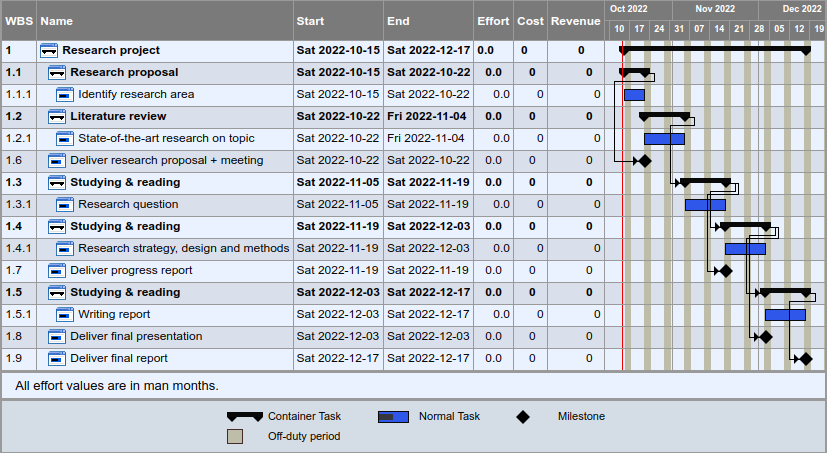
\includegraphics[width=.7\textwidth]{gantt.png}
      \end{figure}
\end{frame} %conclusions

\appendix

\begin{frame}[allowframebreaks]
  \frametitle{参考文献}
  \printbibliography
\end{frame}

\makebottom

\end{document}
